\documentclass[10pt,conference]{IEEEtran}

\usepackage[utf8]{inputenc}
\usepackage{hyperref}
\usepackage{graphicx}
\usepackage{wrapfig}


\begin{document}
\title{\huge Machine Learning - Class Project 1}

\author{
  Marta González, Natalie Bolón, Pau Argelaguet\\
  \small \textit{École Polytechnique Fédérale de Lausanne, Switzerland}
}

\maketitle

\begin{abstract}
This project consists on applying ML techniques on real data from CERN, which are the results of experiments on the Higgs particle (collisions between particles). Given those, the system predicts if a collision has been a result of a Higgs boson (\textit{signal}) or something else (\textit{background}). To do so, data must be preprocessed, then the right algorithm has to be chosen and finally, the hyperparameters that give best results for that algorithms have to be used.
\end{abstract}

\section{Introduction}

The given data has some particularities: for instance, that there are features with values missing (\verb|-999|). That means that just inputting the imported data into an algorithm would give results far from optimal. This fact proves the importance of preprocessing and is independent of the algorithm (and its hyperparameters) chosen: better data will mean better results.

The work of implementing the ML methods has been based on those already implemented on the labs, slightly modified mainly for increasing performance and adapting to required input and output. The main factor for deciding one method or another has been the results of the loss function, using cross validation.

\section{Data preprocess}
In order to deal with data, we first standardize it. The main goal of standardization is scaling the data so that the majority of data is included in a known and bounded interval. Moreover, it ease the detection of possible outliers. Both data sets, train and test, are standardized together due to the fact that they belong to the same underlying distribution, so they receive the same linear transformation. 

They have been considered several transformations to preprocess the data: 
\begin{itemize}
\item Substitution of the values \verb|-999| by the mean of the corresponding feature.
\item Deletion of outliers in the sample.
\item Deletion of the entries in the sample that contain \verb|-999| values.
\item Deletion of the features that contain \verb|-999| values.
\end{itemize}

Applying all these transformations to the data set and to the different methods, it can be seen, using 4-fold cross-validation, that the transformation which gives a smallest error is the standardization together with the deletion of outliers, those data points that have some component far from the mean of the corresponding feature. 

The following figure shows the test errors obtained using 4-fold cross-validation for the different methods and transformations:

\begin{figure}[ht!]
	\centering
	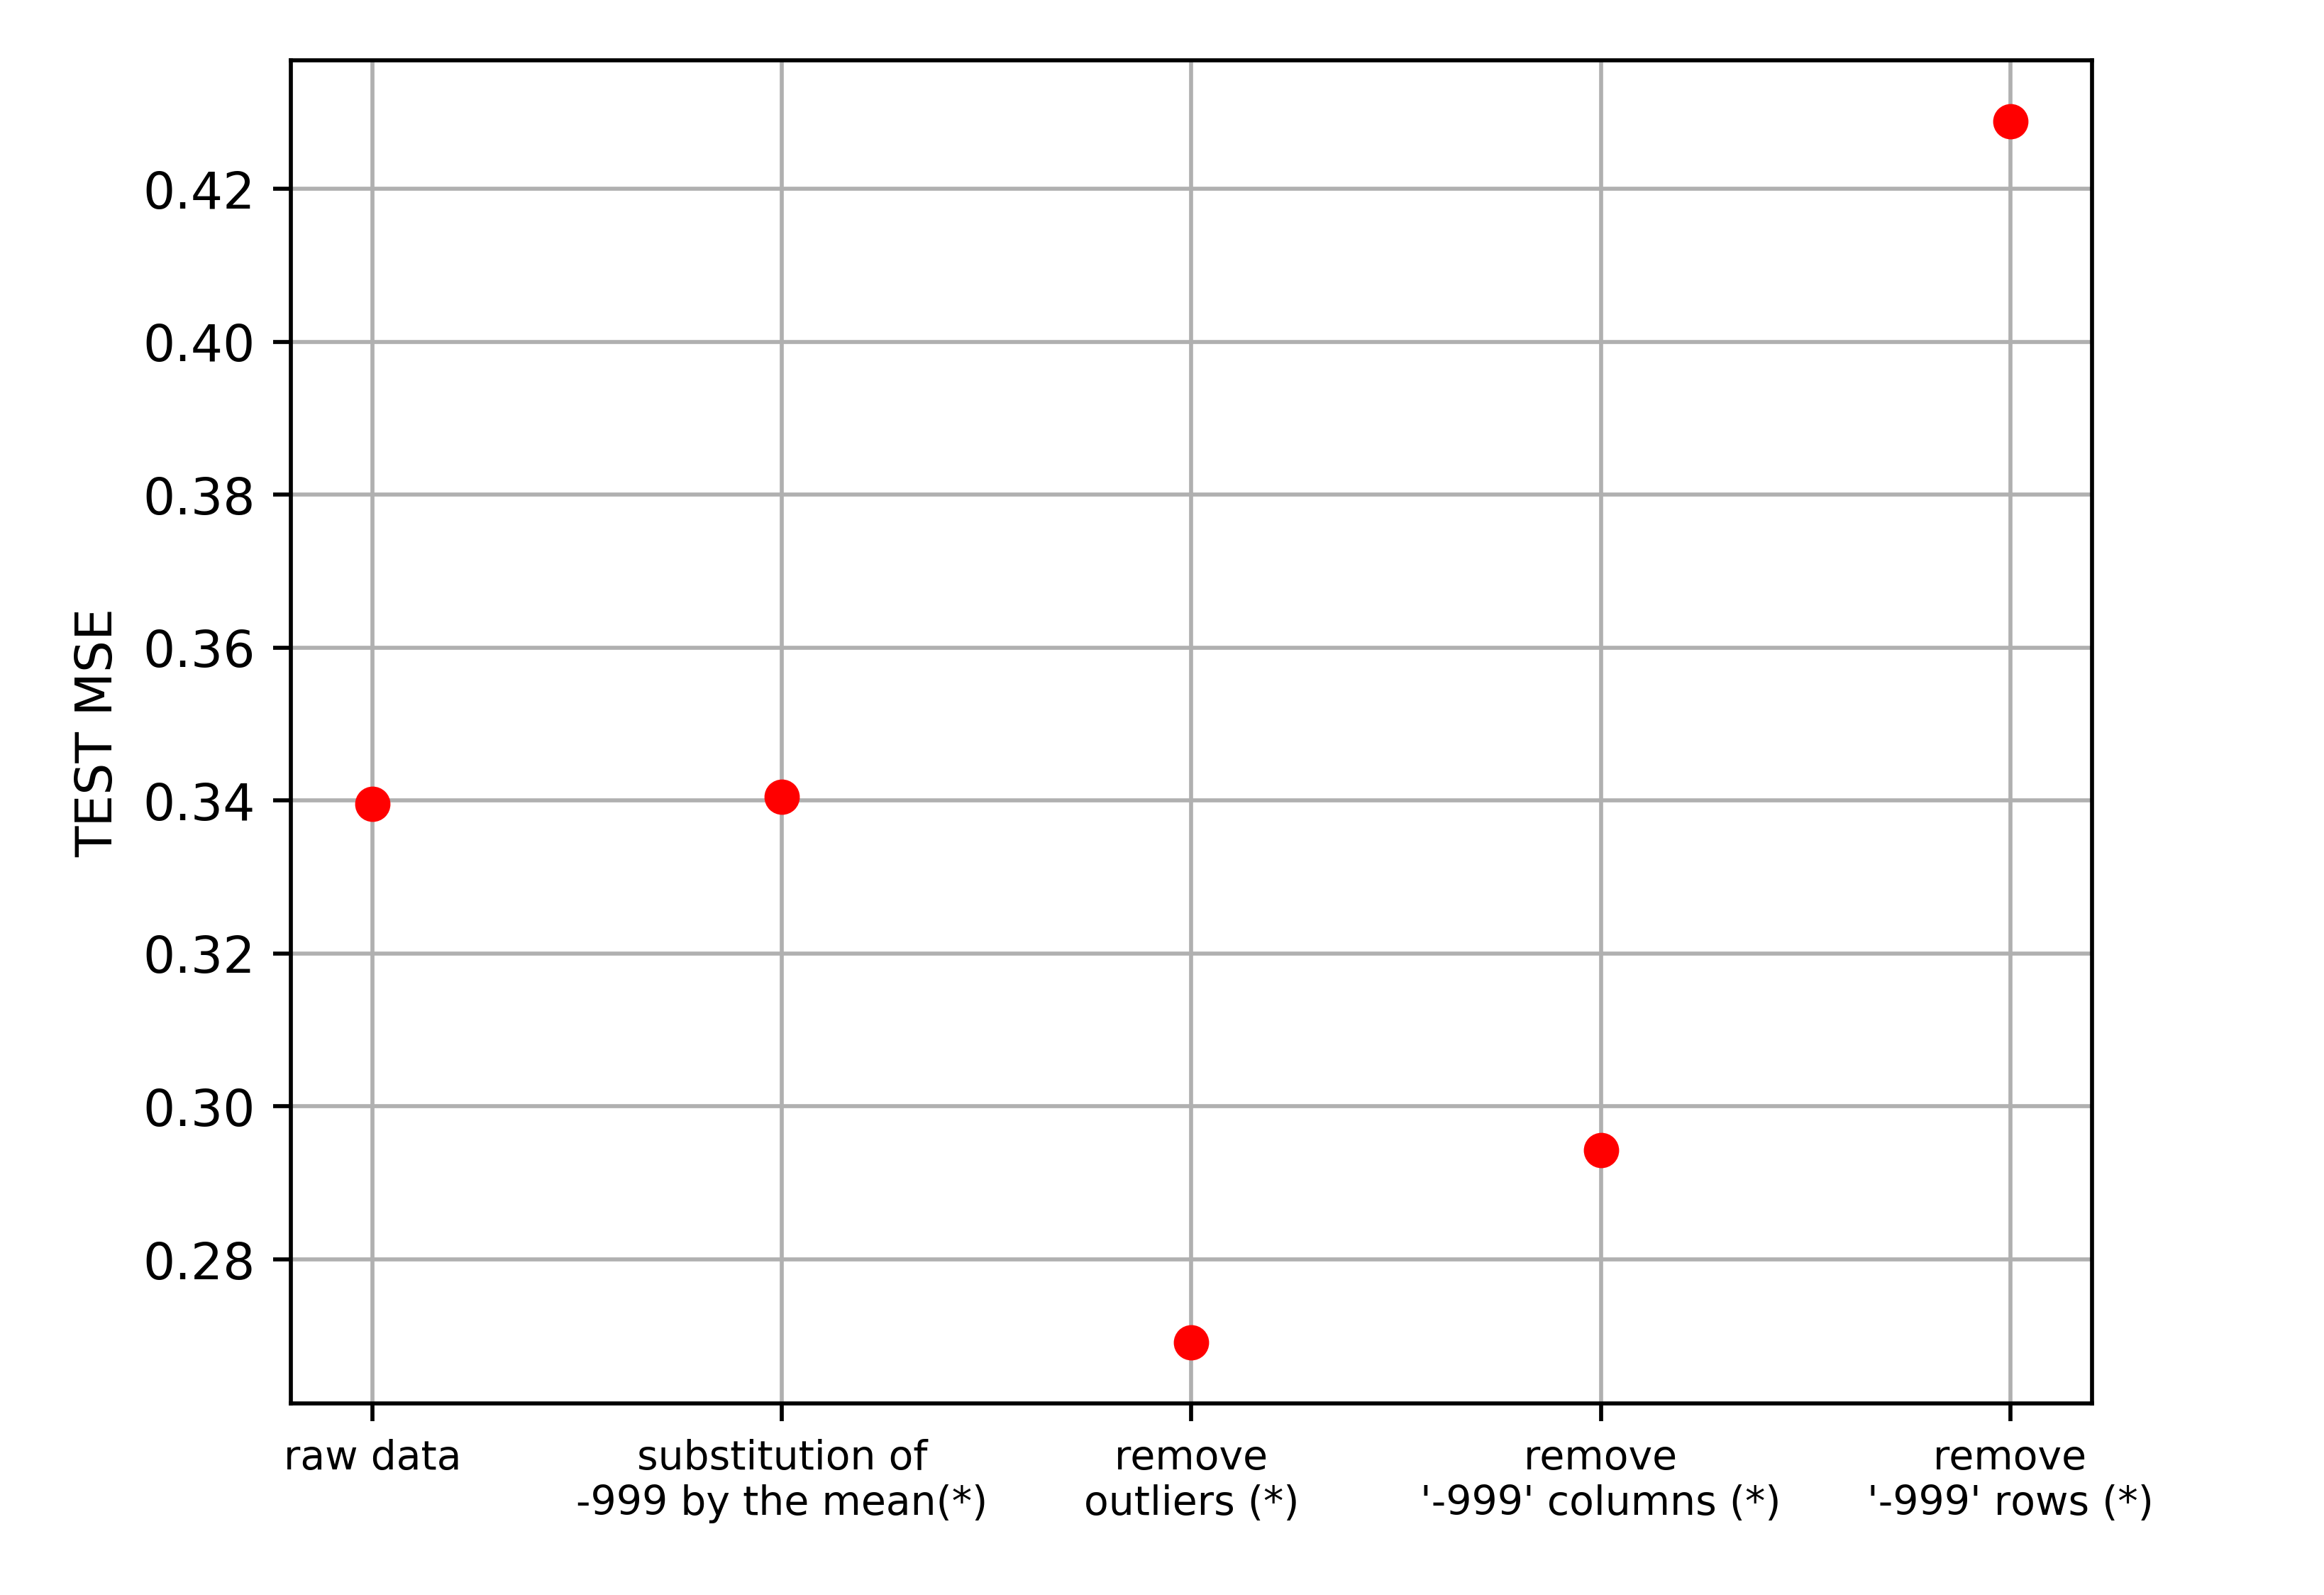
\includegraphics[width=265px]{LEAST_SQUARES_DATA_PRE-PROCESS.png}
	\caption{Test Mean Squared Error for different preprocessing of data and Least Squares}
   \label{figure 1}
\end{figure}

\begin{figure}[ht!]
	\centering
	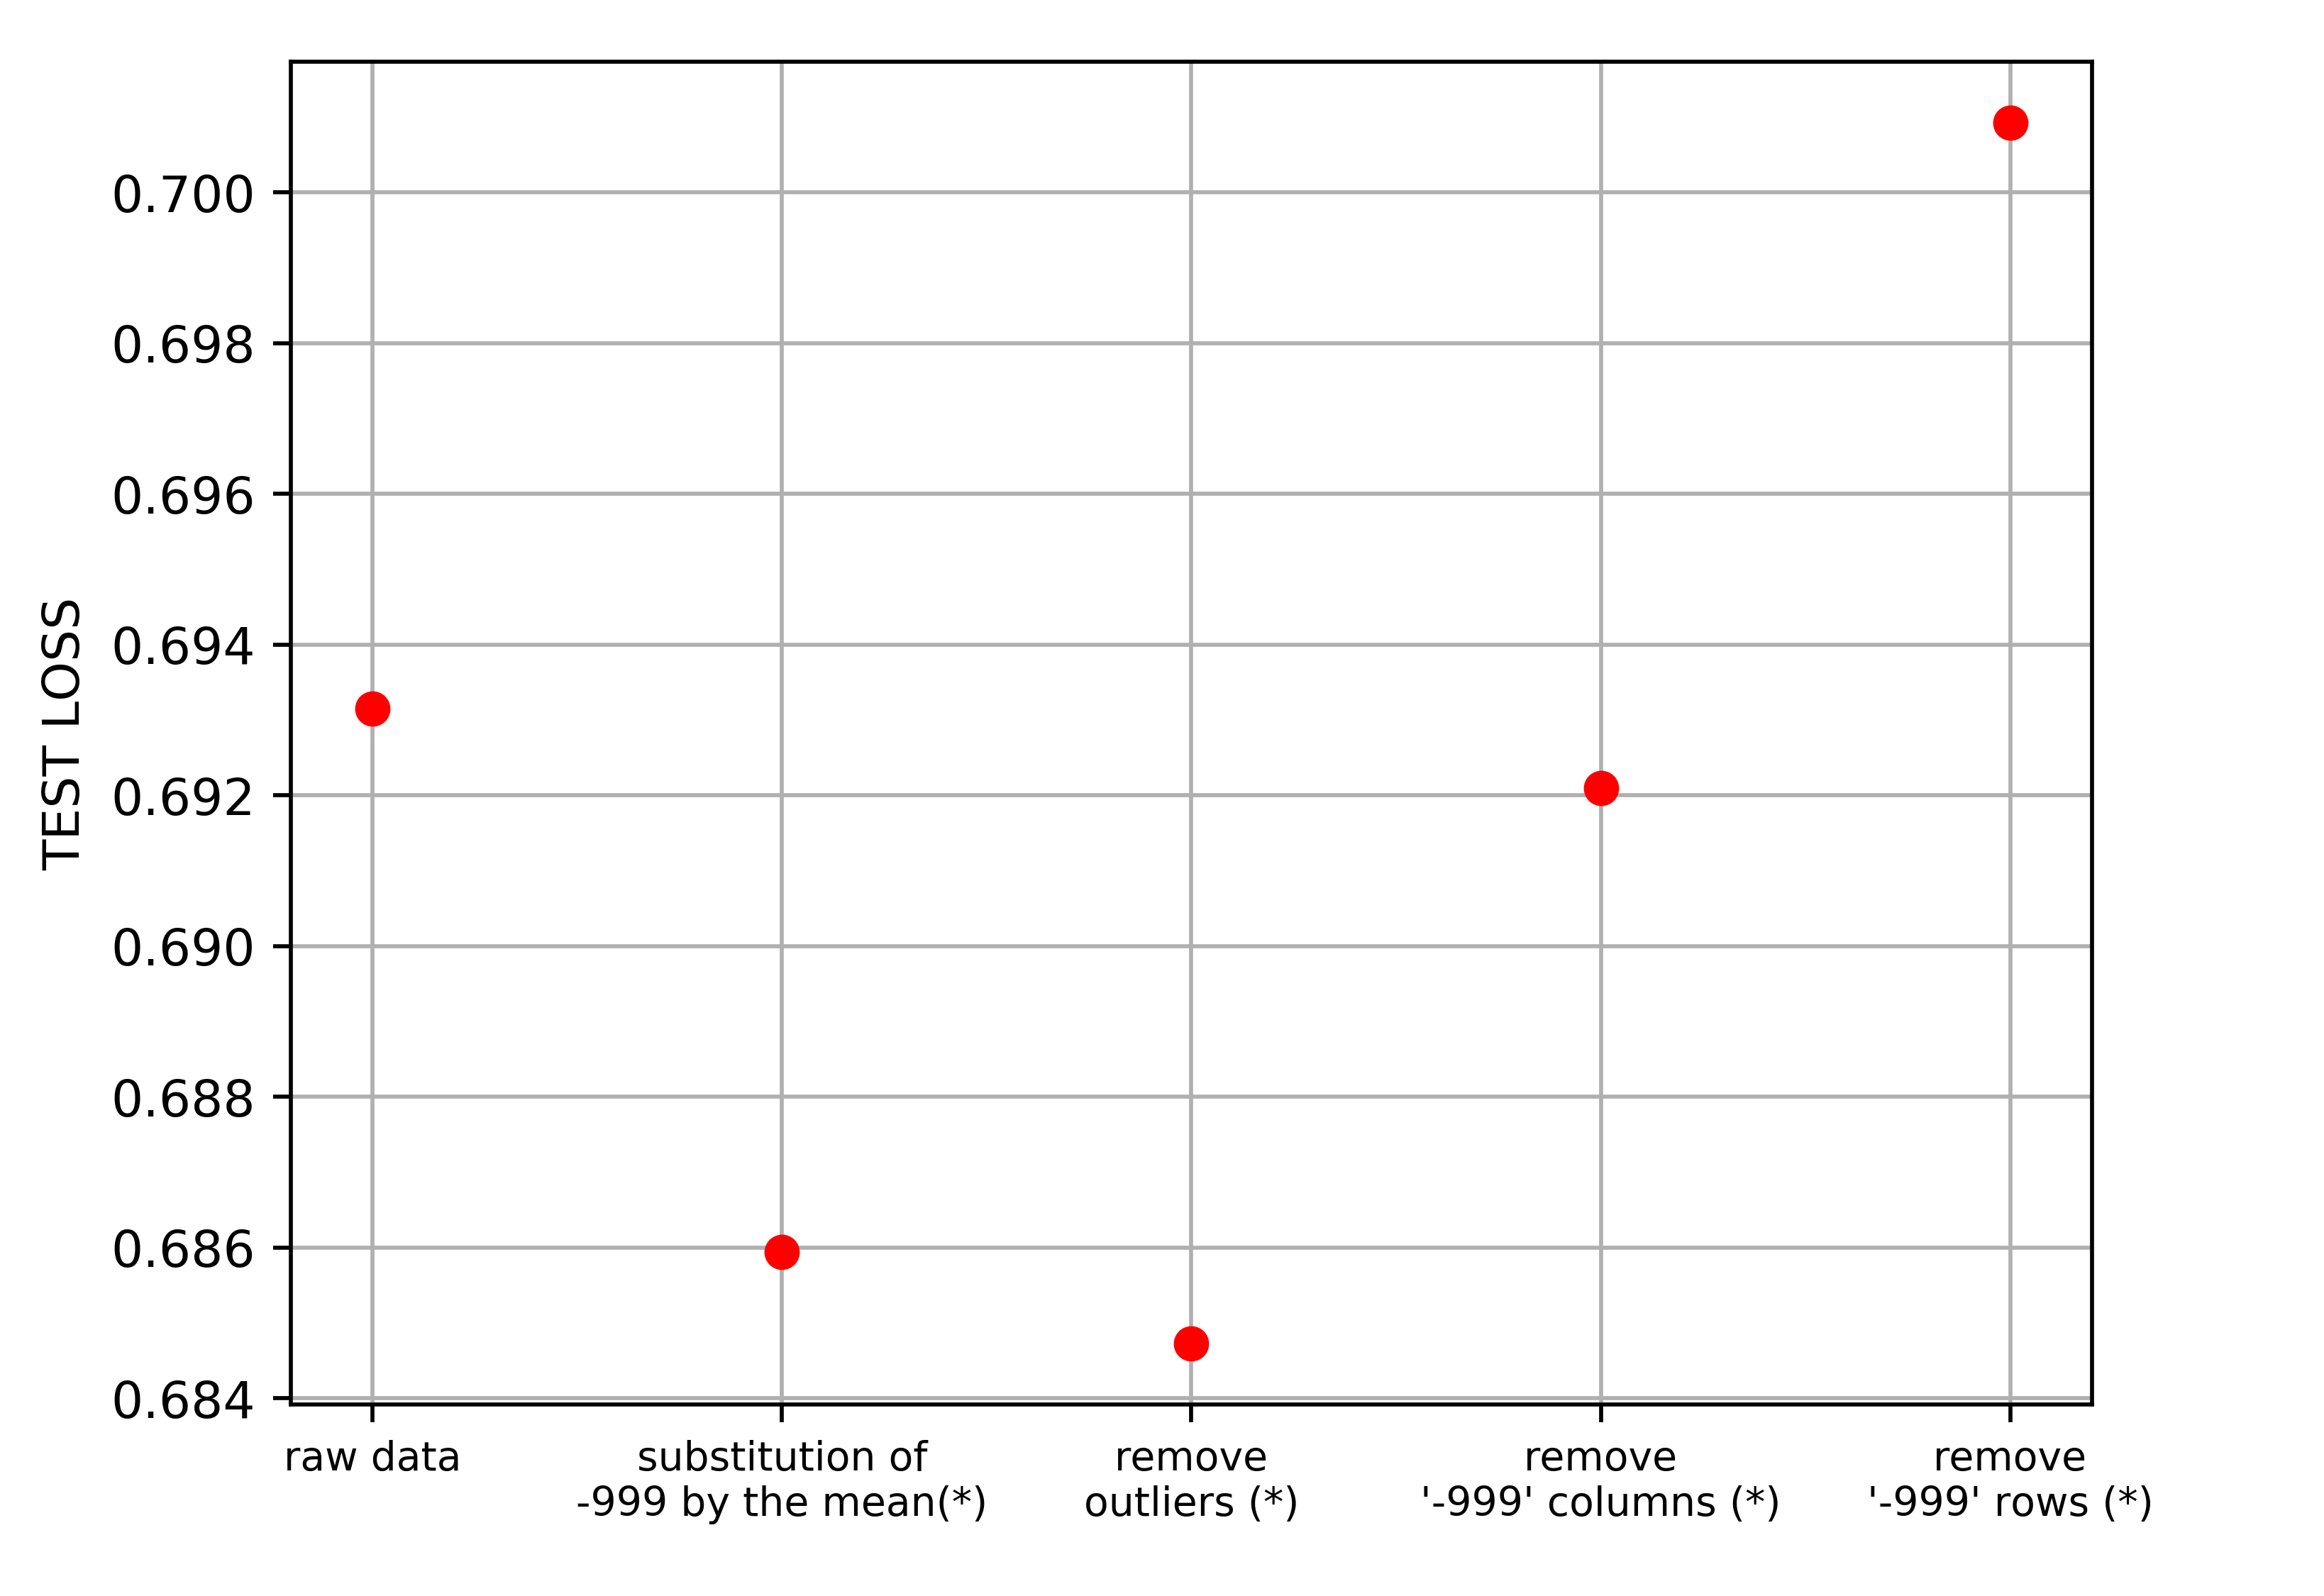
\includegraphics[width=265px]{Log_reg_DATA_PRE-PROCESS.png}
	\caption{Test loss for different preprocessing of data and Logistic Regression. Except from raw data, all other pre-process methods include standardizing the data before. For removing outliers, it also implies substitution of -999 values by their corresponding mean} 
\label{figure 2}
\end{figure}

The results shown in figures \ref{figure 1} and \ref{figure 2} have been obtained after hyperparameter tuning in order to obtain the best result for each method. The process for this tuning will be explained in the following section. 

Both figures show that the error is significantly higher when deleting values of \verb|-999| in rows than when deleting them in columns. This is because these values are concentrated in a few features while they are spread in all the data set. That means that there are many data points that have to be deleted but there are not that many input variables. 

Even so, in both cases too much information is lost in the model. Values \verb|-999| represent unmeasured data so it is feasible to correct their value by the mean. Standardizing the data and changing \verb|-999| by the mean of that input variable gives better results than getting rid of the unmeasured data.

\section{Method selection}

For this project the following methods have been implemented: Linear Regression Gradient Descent, Linear Regression Stochastic Gradient Descent, Least Squares, Ridge Regression, Logistic Regression by GD and Regularized Logistic Regression by GD.

Both Linear Regression by Gradient Descent and by Stochastic Gradient Descent are iterative methods and have been discarded among Least Squares as they will converge to the same optimal result as this last one but with higher computational cost. 

Besides that, Ridge Regression has also been discarded due to the fact that it penalizes high values of the norm of w, and it is useful when the system of equations that has to be solved in Least Squares method does not give a solution. As in this case Least squares gives a solution, Ridge Regression can be ignored. 

Finally, applying to Logistic Regression and Regularized Logistic Regression, both methods have been implemented and studied using the regularized version of them by taking into consideration the case of $\lambda=0$. 

\section{Hyperparameter tuning}

To proceed with the tuning of hyperparameters for each method, 4-fold cross validation has been implemented. Different range of values for each hyperparameter have been considered. 

\subsection{Least Squares}
For Least Squares method, the degree is the only free variable to be determined. To choose its best value, lowest test error criteria has been followed after performing 4-fold cross validation for degrees from 1 to 15. 
As seen in Figure \ref{figure 3}, the best result is achieved by degree 11.

\subsection{Regularized Logistic Regression}
For Logistic Regression method, both degree and $\lambda$ have to be determined. Referring to $\gamma$ value, it has been set initially to 0.1 and it decreases as the loss gets stuck. Using 4-fold cross-validation, the best parameters are $\lambda= 0$ and degree=4, as seen in figure \ref{figure 4}

\begin{figure}[ht!]
	\centering
	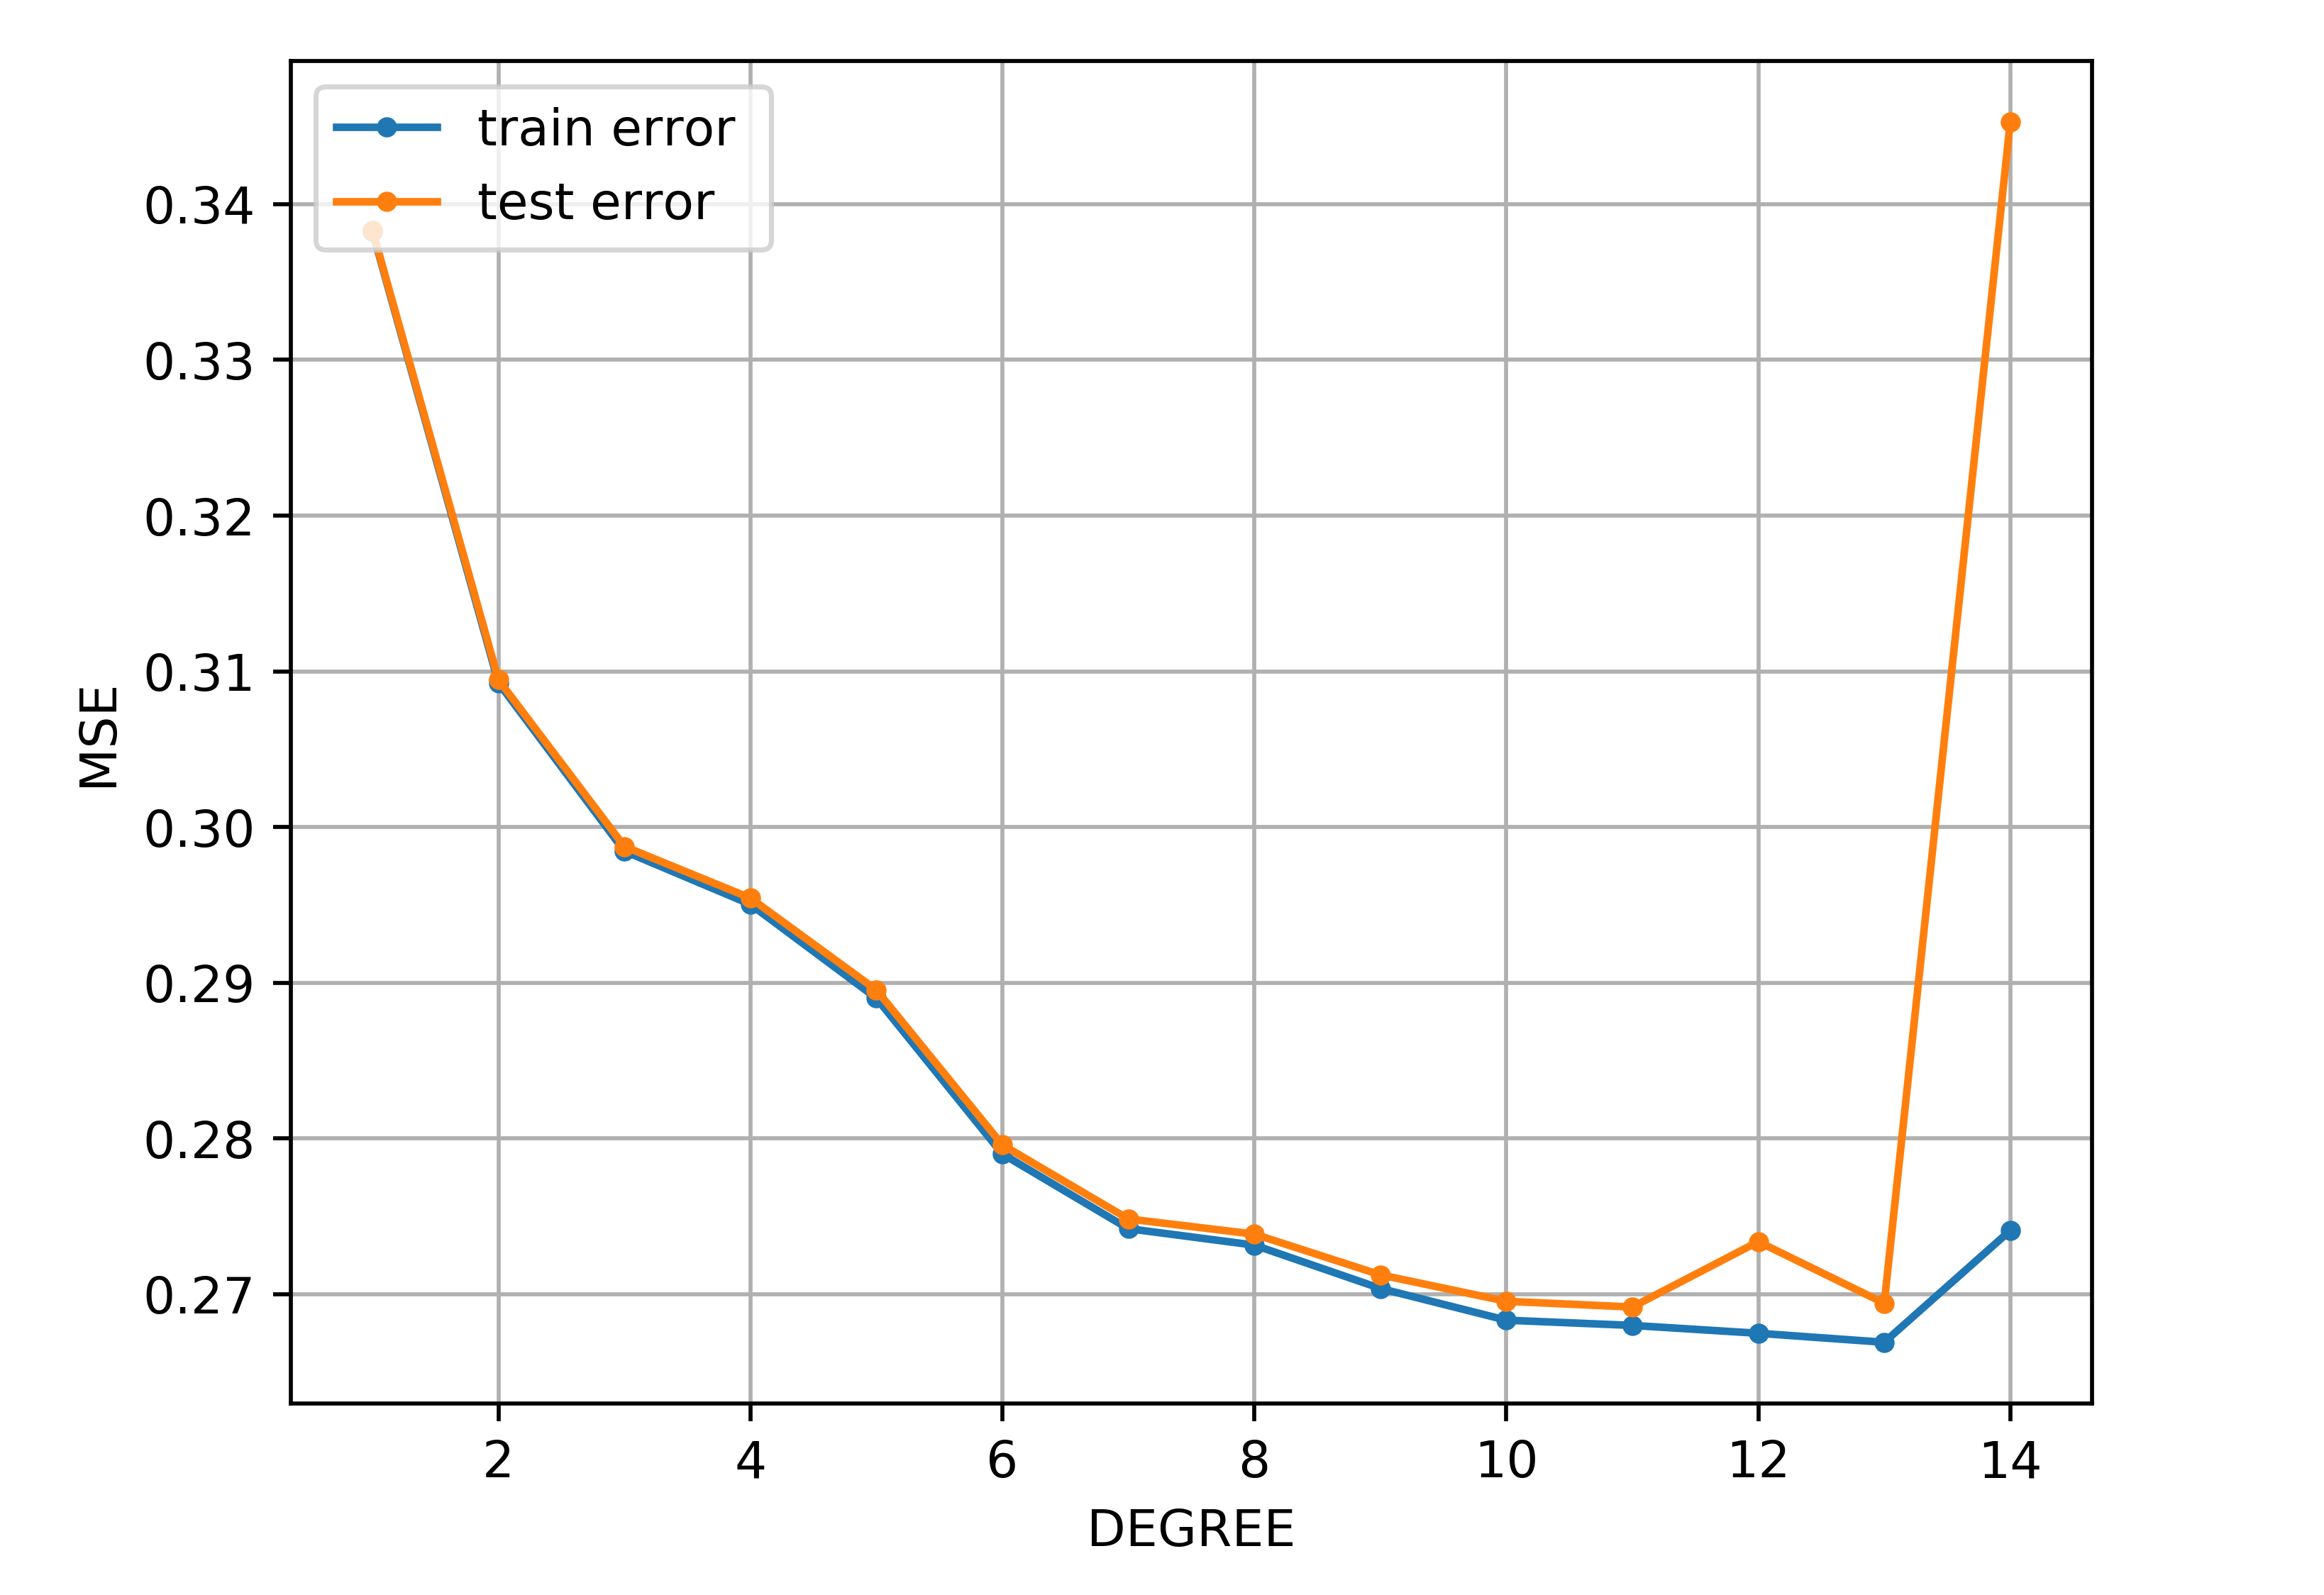
\includegraphics[width=265px]{cross_validation_LS_degress_std.png}
	\caption{Mean Squared Error for Least Squares}
\label{figure 3}
\end{figure}

\begin{figure}[ht!]
	\centering
	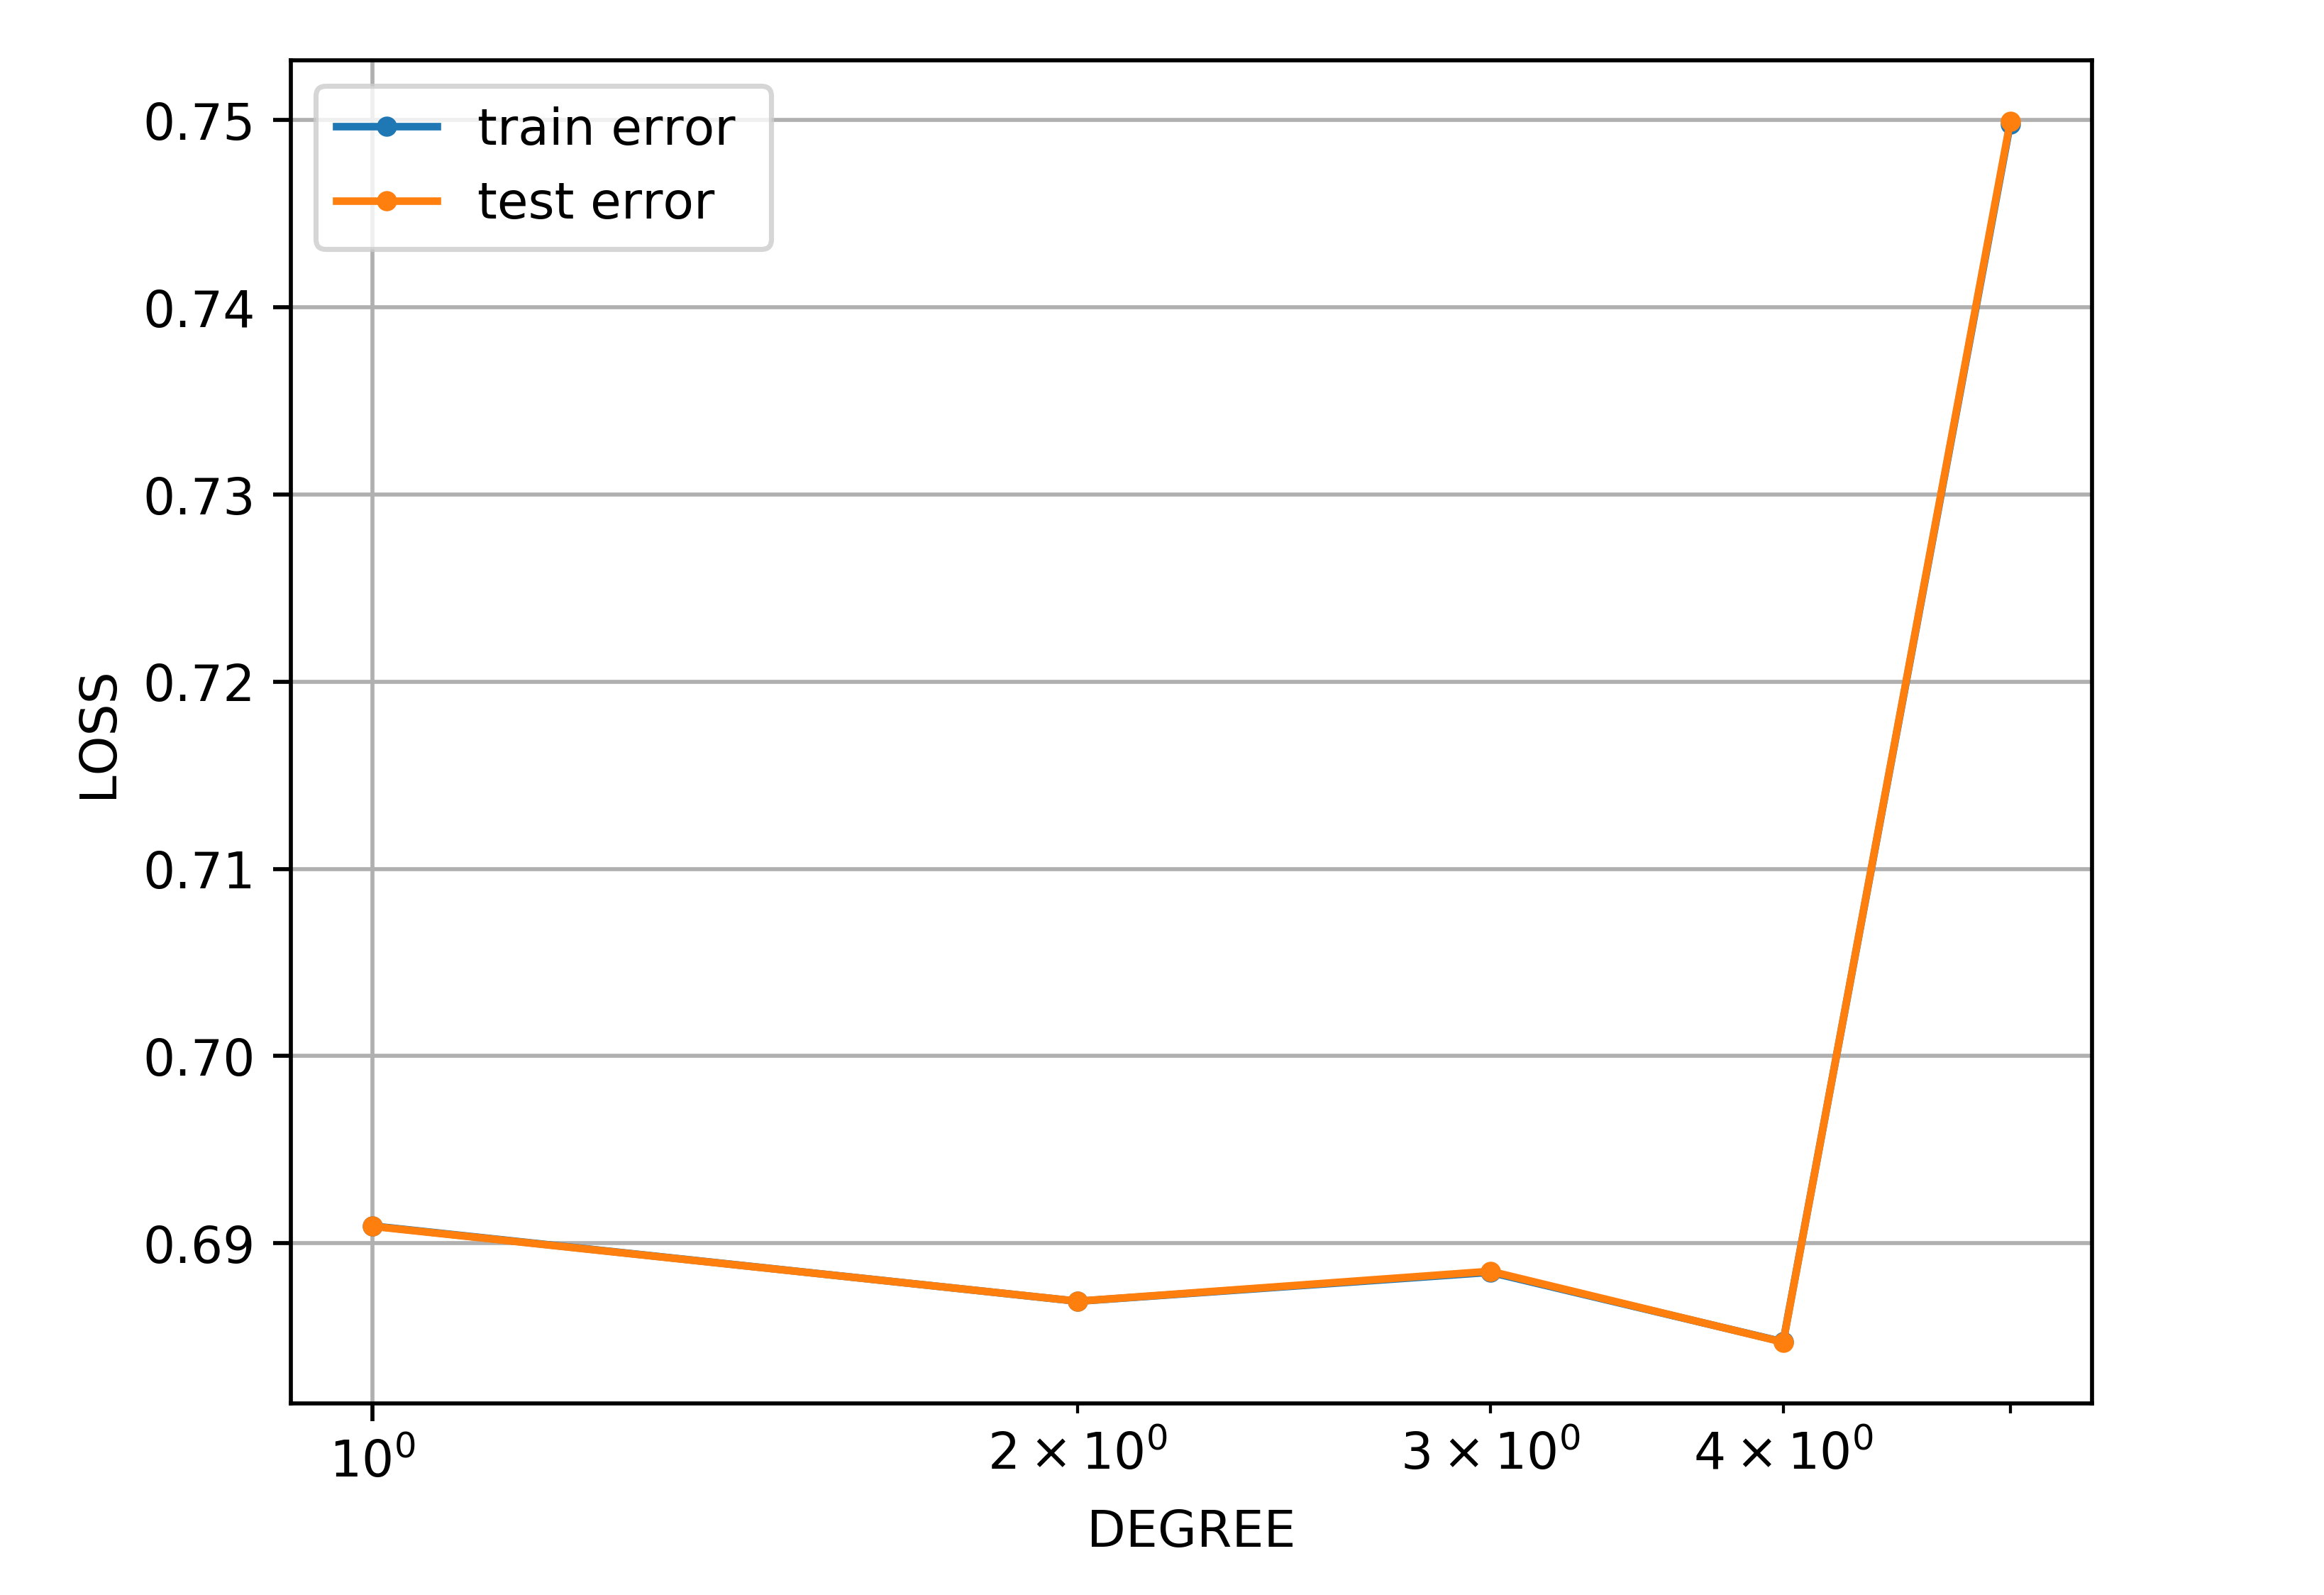
\includegraphics[width=265px]{Reg_Logistic_Regression.png}
	\caption{Loss obtained by Regularized Logistic Regression applied to different degrees using 4-fold cross-validation, with $\lambda=0$ (train error not visible because it is almost identical to test error)}
    \label{figure 4}
\end{figure}
 

\section{Final method and hyperparameters}

In order to decide which method to use for the classification of the data, it is useful to compare the value from a given loss function. As the loss functions associated to Least Squares and Logistic Regression are different, it may be useful to have a new indicator of the accuracy of the method. One example could be the ratio of accurate values classified. Computing this value for the best tuned parameters, by 4-fold cross validation, the results are the following:

\begin{itemize}
\item{}Ratio of accurate predictions for Least Squares: 0.8213
\item{}Ratio of accurate predictions for Logistic Regression: 0.6876
\end{itemize}

\section{Summary}

Finally, the chosen model for this task has been the one given by Least Squares method with degree 11 and outiler threshold 8.5. This model has been validated by 4-fold cross validation and chosen by its low test error and its high ratio of accurate prediction compared to Logistic Regression. 

Moreover, it has been emphasized the importance of data pre-process as it has result in a great decrease of the error independently of the chosen method. Note that since the main goal has been precision of results, computation time hasn't been an issue, therefore, the focus has been on methods that may give better results although taking more time to compute.

\end{document}
